\chapter{Statistics}\label{sec:statistics}

Every scientific investigation starts with a hypothesis that is to be tested empirically. The main objective is to evaluate if the proposed hypothesis agrees or disagrees with observed data, to either accept or reject it against the null-hypothesis which represents a baseline scenario where only known phenomena are presumed to occur. 

A key metric that quantifies this is the p-value that arises within hypothesis testing. Test results of an experiment follow some probability density function. Assuming some hypothesis the p-value is the integrated probability for test results compatible with this hypothesis and ergo measuring the compatibility of the observation to the assumption. In other words if the experiment where to be repeated it gives the probability that the result favors the proposed hypothesis.

In the field of high energy physics a framework has been developed specifically for this task. This section begins to lay out the mathematical fundamentals of the approach and explains its implementation in \textsc{pyhf} \citep{pyhf,pyhf_joss}. The following is based on \citep{cowan2011asymptotic,behnke2013data,pyhf}.
 
\section{Building the likelihood}\label{sec:likelihood}
The statistical model needs to reflect the compatibility of predictions with the observed collision events. This can be quantified by a likelihood $L(\bm{x} | \bm{\phi})$ which is a probability for an observation $\bm{x}$ under a given set of parameters $\bm{\phi}$ that govern the predictions. Given that this is a counting experiment bins of a histogram $\bm{h}=(h_1,...,h_N)$ are the main tool of analysis.

The observation can be subdivided $\bm{x}=(\bm{n},\bm{a})$ into observable histograms $\bm{n}$ and auxiliary measurements. Observable histograms could be the invariant mass of a particle on the other hand auxiliary measurement histograms $\bm{a}$ can be any additional observable that assist in constraining the model. For instance they can be a measurement of a kinematic variable in a phase space region where only background is expected. It should be noted that these auxiliary measurements are not equivalent to the inclusion of uncertainties into the model. The treatment of uncertainties is addressed separately in section \ref{sec:histfactory_model}. 

Another useful splitting for the set of parameters $\bm{\phi}=(\bm{\psi},\bm{\Theta})$ into so-called parameters of interest $\bm{\psi}$ and nuisance parameters $\bm{\Theta}$. For this section only one parameter of interest is considered, the signal strength $\mu$. 

The bin contents can then be expressed in terms of the amount of signal $s_i(\bm{\Theta})$ and background $b_i(\bm{\Theta})$ in bin $i$ that depend on the nuisance parameters. The prediction (expectation value) of the histogram bins of the observable $n_i$ can then be expressed as 
\begin{equation} \label{eq:n_i}
    \langle n_i(\mu,\bm{\Theta})\rangle = \mu s_i(\bm{\Theta}) +b_i(\bm{\Theta}). 
\end{equation}
Similarly for auxiliary measurement bins $a_i$ their expectation value are calculable from some function $u_i(\bm{\Theta})$ modeling some observable and is also dependent on the nuisance parameters
\begin{equation} \label{eq:a_i}
    \langle a_i(\bm{\Theta}) \rangle = u_i(\bm{\Theta}).
\end{equation}
Since this is a counting experiment in which events occur at a constant mean rate and independently of time each bin follows a Poisson distribution
\begin{equation}\label{eq:poisson}
    P(r,k)=\frac{r^k e^{-r}}{k!}.
\end{equation}
$r$ is the expected rate of occurrences which translates as the prediction whereas $k$ are the actual measured occurrences. A likelihood can then be constructed from a product of Poisson probabilities
\begin{equation}\label{eq:likelihood}
    L(\mu,\bm{\Theta})=
    \prod_{j=1}^N \frac{(\mu s_j(\bm{\Theta}) + b_j(\bm{\Theta}))^{n_j}}{n_j !} e^{-(\mu s_j(\bm{\Theta}) + b_j(\bm{\Theta}))}
    \prod_{k=1}^M \frac{u_k(\bm{\Theta})^{a_k}}{a_k!} e^{-u_k(\bm{\Theta})}.
\end{equation}
The last product can also be thought of penalizing the likelihood if e.g. an auxiliary measurement displays a very improbable value for some quantity. To test for a hypothesized value of $\mu$, the best choice according to the Neyman-Pearson lemma \citep{behnke2013data}, is the profile likelihood ratio that reduces the dependence to the parameter(s) of interest
\begin{equation}\label{eq:likelihood_ratio}
\lambda(\mu)=
    \frac{L(\mu,\hat{\hat{\bm{\Theta}}})}
    {L(\hat{\mu},\hat{\bm{\Theta}})}.
\end{equation}
The denominator is the unconditional maximum likelihood estimate so that $\hat{\mu}$ and $\hat{\bm{\Theta}}$ both are free to vary to maximize $L$, whereas the numerator is the found maximum likelihood conditioned on some chosen $\mu$ and the set of nuisance parameters $\hat{\hat{\bm{\Theta}}}$ that maximize the likelihood for that particular $\mu$. This definition gives $0 \leq \lambda \leq 1$ where $\lambda = 1$ corresponds to perfect agreement of the hypothesized value of $\mu$ to the model.

\section{From test statistic to p-value}
To test for alternative hypotheses it is useful to transform the profile likelihood into a test statistic
\begin{equation}
    t(\mu)=-2\ln \lambda(\mu).
\end{equation}
This translates to $t \rightarrow 0$ as increasing agreement and $t \rightarrow \infty$ as decreasing agreement to the model. A right-tail p-value can then be calculated from the probability density function of the test statistic: \ac{pdf}$(t) = f(t | \mu)$
\begin{equation}\label{eq:p-value}
    p= \int_{t_\text{obs}}^{\infty} 
    f(t | \mu) \mathrm{d}t
\end{equation}
$t_\text{obs}$ is the test statistic $t$ evaluated at the observed data which means replacing the predictions in the likelihood of the numerator of equation \ref{eq:likelihood_ratio} with the values observed in data. Similar to the \ac{pdf} of a standard normal distribution the \ac{pdf} in this context quantifies how probable a particular value of the test statistic $t$ is under a fixed value of the signal strength. This essentially measures how frequently a particular value of $t$ occurs in comparison to all other possible values that $t$ can have.

This form is particularly useful due to existing approximations for $f(t | \mu)$ \citep{cowan2011asymptotic}. Wald \citep{wilks1938large} proved that for the null hypothesis in the large sample limit, the test statistic follows a normalized sum of squared distances between the tested parameters of interest $\mu$ and its maximum likelihood estimate $\hat{\mu}$. 
\begin{equation}
    t(\mu)=-2\ln \lambda(\mu)=
     \left(\frac{\mu-\hat{\mu}}{\sigma_{\hat{\mu}}} \right)^2
    + \mathcal{O}(\frac{1}{\sqrt{N}}).
\end{equation}
The maximum likelihood estimate $\hat{\mu}$ is in the large sample limit normally distributed around their true values $\mu'$ with standard deviation $\sigma_{\hat{\mu}}$. This is the definition of a non-central $\chi$-squared distribution with one degree of freedom. It can be shown that the \ac{pdf} of $t$ can be described by \red{cite}
\begin{equation}\label{eq:chi-square}
    f(t | \mu)=\frac{1}{2\sqrt{t}}\frac{1}{\sqrt{2\pi}}
    \left[
\exp\left(-\frac{1}{2}\left(\sqrt{t}+\sqrt{\Lambda}_\mu\right)\right)
+
\exp\left(-\frac{1}{2}\left(\sqrt{t}-\sqrt{\Lambda}_\mu\right)\right)
\right],
\end{equation}
with non-centrality parameter as the normalized distance between tested and
true parameter of interest value
\begin{equation}
    \Lambda_\mu=\frac{(\mu-\mu')^2}{\sigma^2}.
\end{equation}
Figure \ref{fig:test_stat_example} illustrates the different steps. Being able to calculate p-values allows now to state how likely it is that the proposed hypothesis is reflected by the observed data. In other words, the p-value represents the probability, how incompatible the proposed hypothesis (prediction) is with the observation.

In the scientific community a widely accepted threshold for this is a p-value of 0.05. Though particle physicists only claim discovery of a new phenomenon for $p$ < \qty{2.87e-7}{} corresponding to 5 standard deviations of the standard normal distribution and exclude hypotheses if the p-value is not below 2 standard deviations of the standard normal distribution $p$ $\lesssim$ \qty{0.05}{}. One caveat here is that this particular form of $t$ assumes $\mu$ can also be negative, which can be non-physical depending on the impact of a new process. Test statistics and their \acp{pdf} approximations considering the different cases are covered in \citep{cowan2011asymptotic}. 
\begin{figure}
    \centering
    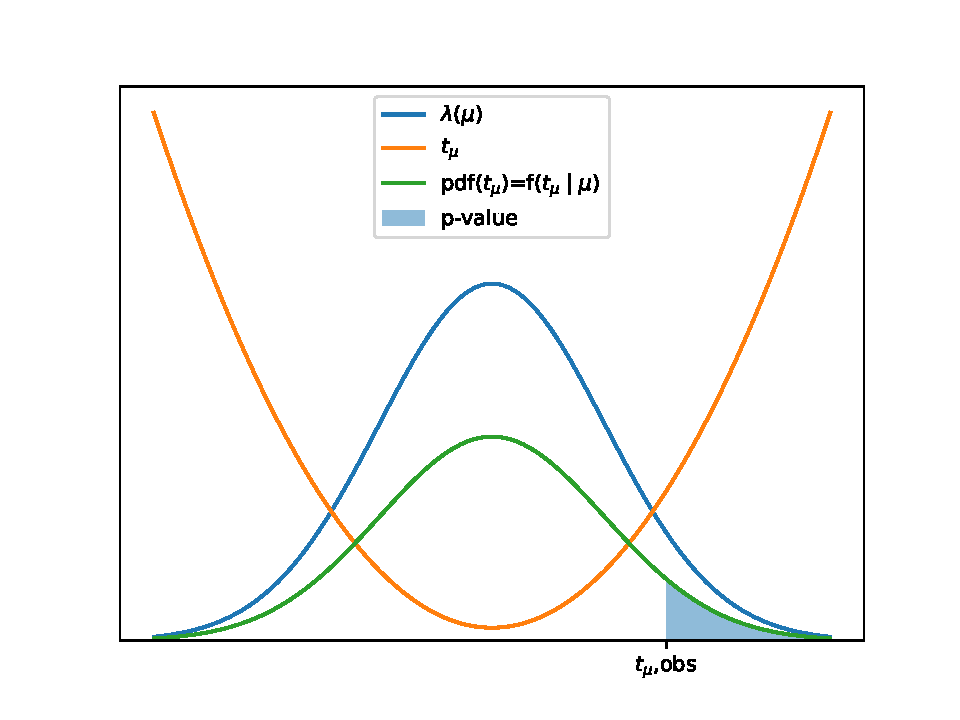
\includegraphics[width=0.8\textwidth]{test_stat_example.pdf}
        \caption[]{A sketch to follow the steps to calculate p-values. (\textbf{left}) The profile likelihood (\hexbox{1f77b4}) has essentially some hill-like form with a maximum at ${\lambda(\hat{\mu},\hat{\bm{\Theta}})}$, $t$ (\hexbox{ff7f0e}) is $-2\mathrm{ln}(\lambda)$. (\textbf{right}) For one parameter of interest in the large sample limit $f(t | \mu)$ follows a non-central chi-squared distribution with one degree of freedom, equation \ref{eq:chi-square}. The blue shaded area under the \acp{pdf} is a right hand sided p-value.}
    \label{fig:test_stat_example}    
\end{figure}

\section{The CL$_s$ value}\label{sec:cls}

Particle physicists are usually interested in two things when making statistical tests for the discovery of new phenomena: how well is the modeling of backgrounds (things we know) and whether there is evidence in the observations for a new phenomenon. This means one needs to test two hypotheses: a background only ($b$) and a signal plus background ($s+b$) hypothesis. Each will result in a p-value of their own. For example, $p_{b}=0$ would mean that the backgrounds are perfectly reflected by the observations and a $p_{s+b} < 0.05$ could be a sign of e.g. new physics. To combine these two metrics into a single score, particle physicists came up with the pseudo Confidence Level/p-value called CL$_s$ incorporating also the goodness of the modeling of the backgrounds 
\begin{equation}
    \mathrm{CL}_s=\frac{p_{s+b}}{1-p_{b}}=
    \frac
    {\int_{t_\text{obs}}^{\infty} 
    f(t_{s+b} | \mu) \mathrm{d}t}
    {1-\int_{t_\text{obs}}^{\infty} 
    f(t_{b} | \mu) \mathrm{d}t}.
\end{equation}
Intuitively the numerator is again just the value for the alternative hypothesis whereas the denominator penalizes CL$_s$ if the modeling of the backgrounds is not reflected in the observations. This can also be understood visually from the first figure of the paper that introduced the CL$_s$ quantity \citep{read2002presentation} (see description of fig. \ref{fig:cls}).
\begin{figure}
    \centering
    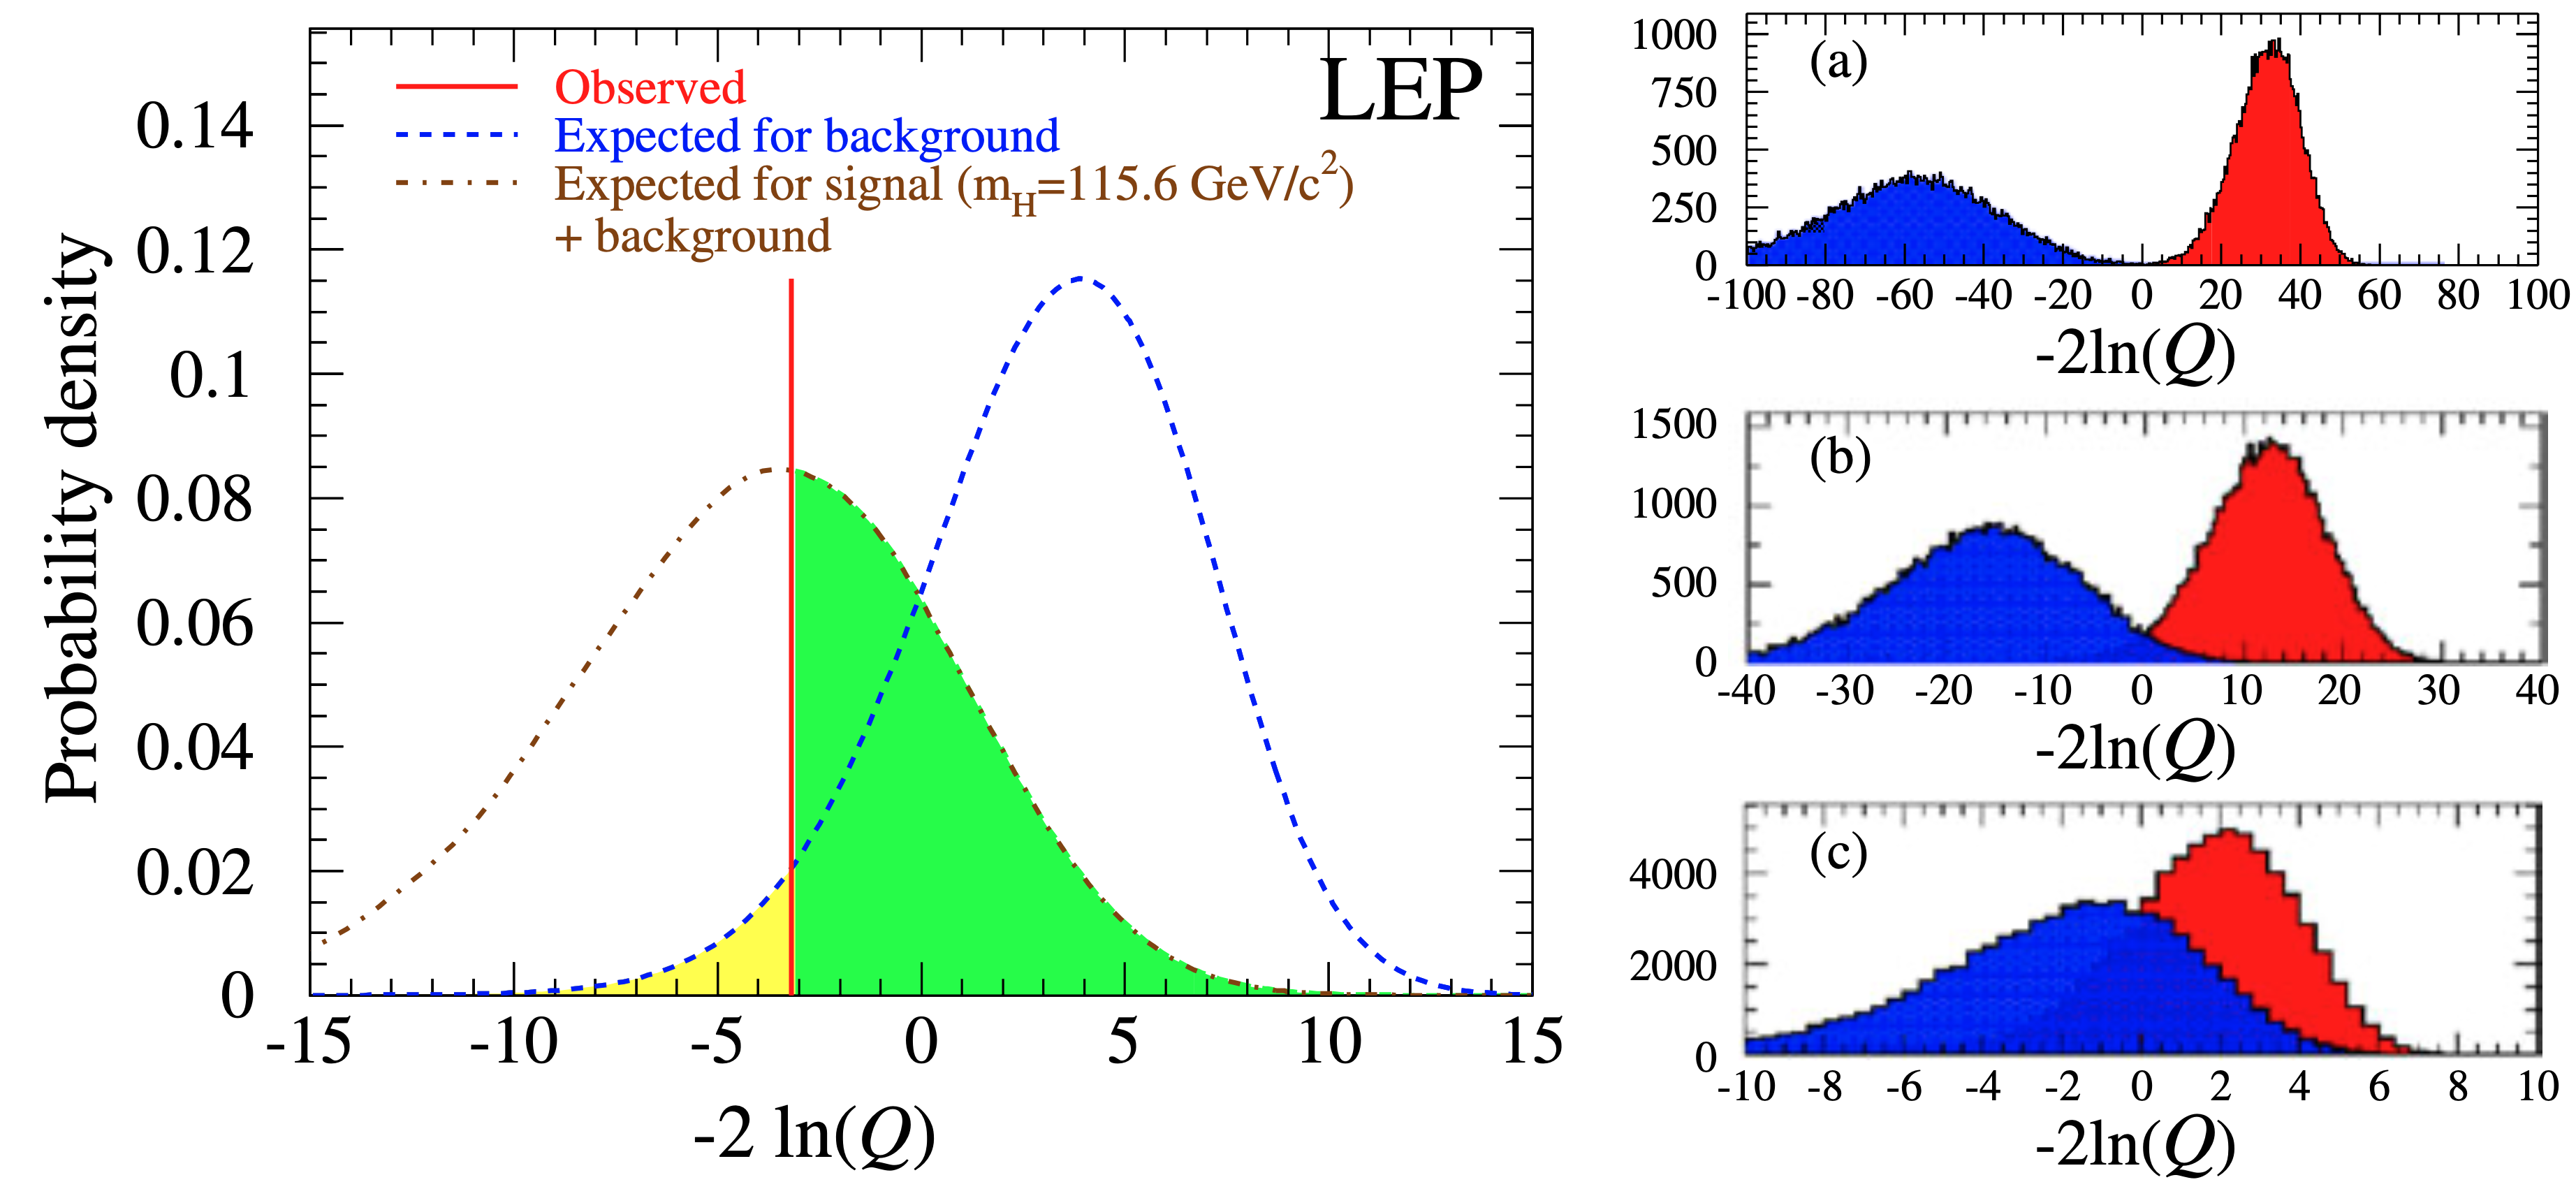
\includegraphics[width=1\textwidth]{cls.png}
        \caption[]{Probability density functions of test statistics from a Higgs search at LEP illustrating the calculation of p-values ($\lambda$ becomes $Q$). (\textbf{left}) The \acp{pdf}'s of the test statistic $f(t | \mu)$ of the signal + background ({\color[HTML]{804000}{$\bm{\diagup}$}}) and background ({\color[HTML]{2100FF}{$\bm{\diagup}$}}) only hypotheses. The p-value is calculated by integration from $t_\text{obs}$ (the red observed line ({\color[HTML]{FF0000}{$\bm{\diagup}$}})) to infinity (see eq. \ref{eq:p-value}). The green shaded area (\hexbox{00FF00}) corresponds to $p_{s+b}$ whereas the yellow area (\hexbox{FDFF02}) corresponds to $1-p_b$ since the integral over one whole \acp{pdf} is 1. (\textbf{right}) Degradation of search sensitivity from (a) to (c). Note that the colors of the \acp{pdf}'s change here to signal + background (\hexbox{2100FF}) and background only (\hexbox{FF0000}). For example putting the observation ($t_\text{obs}$) on the x-axis at 0 in these plots, one would get for plot (a) $p_{b}\approx 1$ and $p_{s+b}\approx 0$ resulting in a CL$_s\approx 0$, whereas with increasing overlap the CL$_s$ value increases and the sensitivity decreases.
        Taken from \citep{read2002presentation}.}
    \label{fig:cls}    
\end{figure}



\section{The \textsc{HistFactory} model}\label{sec:histfactory_model}

A model used widely to build a likelihood as described in section \ref{sec:likelihood} is called HistFactory \citep{cranmer2012histfactory} and is implemented within \textsc{pyhf} \citep{pyhf}. This section is based on the introduction to the model within the documentation of \textsc{pyhf}. HistFactory reduces the building of a likelihood into a small number of basic components. For this purpose, it is again useful to think of another splitting of the model parameters $\bm{\phi}$ into

\newcommand{\freeset}{\bm{\eta}}
\newcommand{\constrset}{\bm{\chi}}
\newcommand{\singleconstr}{\chi}
\newcommand{\channelcounts}{\bm{n}}
\newcommand{\auxdata}{\bm{a}}
\newcommand{\poiset}{\bm{\psi}}
\newcommand{\nuisset}{\bm{\theta}}
\newcommand{\fullset}{\bm{\phi}}
\newcommand{\singlefull}{\phi}


\begin{equation}
 L(\bm{x}|\fullset) \quad=\quad
 L(\bm{x}|\overbrace{\poiset}^{\llap{\text{parameters of interest}}},\underbrace{\nuisset}_{\llap{\text{nuisance parameters}}}) \quad=\quad
 L(\bm{x}|\overbrace{\freeset}^{\rlap{\text{free}}},\underbrace{\constrset}_{\rlap{\text{constrained}}}) 
\end{equation}
free parameters $\freeset$ and constrained parameters $\constrset$. Free parameters are free to choose in the model and can be for example a cross-section of a process. Constrained parameters are used to incorporate uncertainties into the likelihood to constrain it. Further there might be several histograms of an observable, for example measured in orthogonal kinematic regions, that are called channels $c$. Bins have the index $b$ here and constraint terms are denoted $c_{\singleconstr}$. With that the likelihood can be described by 
\begin{equation}
L(\channelcounts, \auxdata \,|\,\freeset,\constrset) = \underbrace{\color{blue}{\prod_{c\in\mathrm{\,channels}} \prod_{b \in \mathrm{\,bins}_c}\textrm{Pois}\left(n_{cb} \,\middle|\, \nu_{cb}\left(\freeset,\constrset\right)\right)}}_{\substack{\text{Simultaneous measurement}\\%
\text{of multiple channels}}} \underbrace{\color{red}{\prod_{\singleconstr \in \constrset} c_{\singleconstr}(a_{\singleconstr} |\, \singleconstr)}}_{\substack{\text{constraint terms}\\%
\text{for }\text{auxiliary measurements}}}.
\end{equation}
The $n_{cb}$ is the observation and $\nu_{cb}(\freeset,\constrset)$ the prediction. The $c_{\singleconstr}(a_{\singleconstr} |\, \singleconstr)$ are calculated from auxiliary measurements $a_{\singleconstr}$ (the uncertainties) to constrain the parameter $\singleconstr$ and can be any function (e.g. Gaussian, Poissonian,...) the parameter/uncertainty is believed to be distributed.

The prediction is a sum of nominal bin counts\footnote{also called rates, like in the definition of a Poisson distribution} $\nu_{scb}^0$ over all samples $s$ (e.g. $t\overline{t}$, multijet-background, etc.). These nominal bin counts are subject to uncertainties. Therefore the bin counts can be varied within the bounds of these uncertainties. However the effect of this modification to the likelihood must be taken into account which is through the constraint terms. These penalize the likelihood the larger the modification to a nominal value becomes. The $\nu_{scb}^0$ are varied with multiplicative $\kappa_{scb}$ and additive modifiers $\Delta_{scb}$ 
\begin{align}
    \nu_{cb}\left(\fullset\right) &= \sum_{s\in\mathrm{\,samples}} \nu_{scb}\left(\freeset,\constrset\right)\\ 
    &= \sum_{s\in\mathrm{\,samples}}\underbrace{\left(\prod_{\kappa\in\,\bm{\kappa}} \kappa_{scb}\left(\freeset,\constrset\right)\right)}_{\text{multiplicative modifiers}}\, 
    \Bigg(\nu_{scb}^0 + \underbrace{\sum_{\Delta\in\bm{\Delta}} \Delta_{scb}\left(\freeset,\constrset\right)}_{\text{additive modifiers}}\Bigg).
\end{align}
The different types of modifiers are explained in section \ref{sec:modifiers} and the constraint terms $c_{\singleconstr}$ in section \ref{sec:constraint_terms}.

Why this is useful can be seen by considering one uncertainty to a nominal bin count estimate $\nu_{scb}^0$. By modifying $\nu_{scb}^0$ with a factor $\kappa$ in a way that increases the Poisson probability while the corresponding constraint term $c_\kappa(\kappa)$ stays around 1, it can be beneficial for the goal of maximizing the likelihood. This means the most likely/compatible value to the observed data within the modeling of the uncertainties can be found. 

\section{The Modifiers}\label{sec:modifiers}
In HistFactory there are by convention four types $\{\lambda,\mu,\gamma,\alpha\}$ of such multiplicative rate modifiers that are explained in this section. There are \textbf{free rate modifiers $\lambda$ and $\mu$} that affect all bins equally, like the cross-section of a process or the luminosity 
\begin{equation}
    \nu_{scb}(\mu)=\mu \nu_{scb}^0.
\end{equation}
These are bin-independent normalization factors and preserve the shape of the histogram. 
Further there are \textbf{bin-wise modifiers} $\gamma_b$ (uncorrelated shape)
\begin{equation}
    \nu_{scb}(\gamma_b)=\gamma_b \nu_{scb}^0.
\end{equation}
These are useful for example to include uncertainties of a per bin data-driven background estimate. This type without a constraint term is not of much use as if there is only one sample or channel, the fit would always match the data perfectly.
In addition there exist \textbf{interpolation parameters $\alpha$} (shape factors) that enter the modeling through an interpolation function $\eta$ instead of being the factor itself. They exist in multiplicative versions 
\begin{equation}
    \nu_{scb}(\alpha)=\eta(\alpha) \nu_{scb}^0,
\end{equation}
and additive versions
\begin{equation}
    \nu_{scb}(\alpha)=\nu_{scb}^0 + \eta(\alpha).
\end{equation}
This is useful to include systematic uncertainties. In a typical ATLAS analysis usually one knows the one standard deviation of a bin count $\eta_{-1}=\nu_{scb}^\mathrm{1down}$ and $\eta_{1}=\nu_{scb}^\mathrm{1up}$ to the nominal value $\nu_{scb}^0$ of an uncertainty. These are used to construct interpolation functions that modify the nominal value with a nuisance parameter that is also used to apply a penalization $c_\alpha$ according to the modeling of the uncertainty.

In HistFactory there exists four of such interpolation functions. For those exist an identity operator 
\begin{equation}
    \eta_0=\eta (\alpha=0) =
    \begin{cases}
        1 ,& \text{multiplicative modifier, } (\kappa) \\
        0 ,& \text{additive modifier, } (\lambda).
    \end{cases}
\end{equation}
One example of these interpolation functions that scales the bin count linearly over the known deviations $\eta_{-1}=\nu_{scb}^\mathrm{1down}$ and $\eta_{1}=\nu_{scb}^\mathrm{1up}$ is
\begin{equation}
    \eta_\mathrm{linear}(\alpha)=
    \begin{cases}
        \alpha(\eta_0 - \eta_1) ,& \alpha>0\\
        \alpha(\eta_0 - \eta_{-1}) ,& \alpha<0
    \end{cases}
\end{equation}
This is illustrated in fig. \ref{fig:interp_func}(a). For the other ones see e.g. \citep{heinrich2019searches}. It is noted that $\alpha$ is the nuisance parameter and not the function $\eta(\alpha)$ and there is an associated constraint term $c_\alpha$ to each $\alpha$.
\begin{figure}
    \centering
    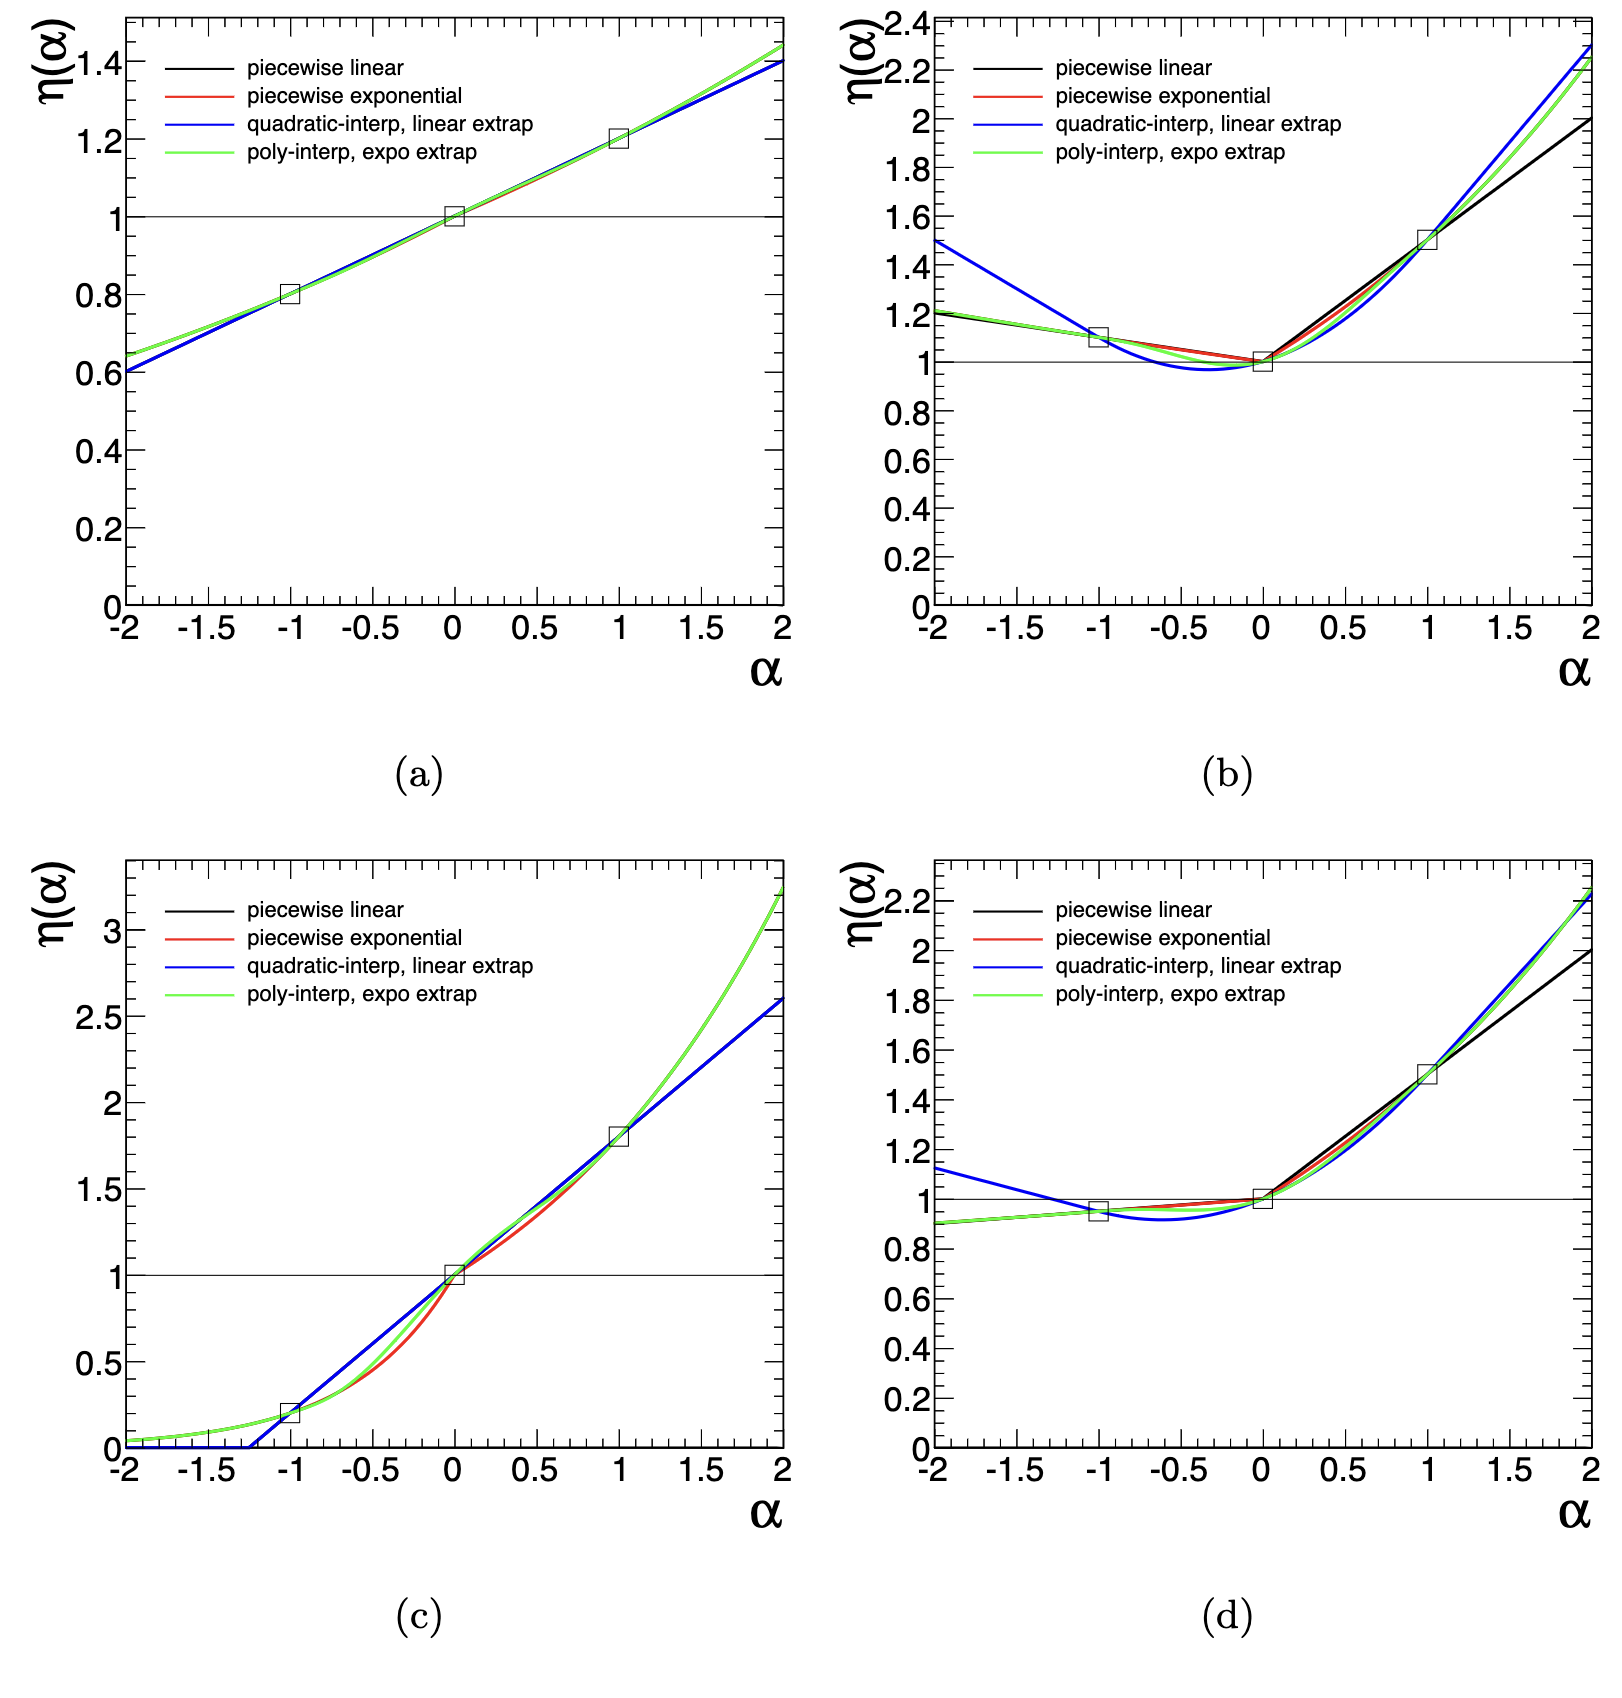
\includegraphics[width=.8\textwidth]{interp_func.png}
        \caption[]{The four interpolation functions $\eta(\alpha)$ for different up and down standard deviation values. For example in (a) the bin count will be scaled with a factor of 0.8 for an $\alpha=-1$ (1.2 for an $\alpha=1$). From \citep{cranmer2012histfactory}.}
    \label{fig:interp_func}    
\end{figure}

\section{The constraint terms}\label{sec:constraint_terms}
Uncertainties are modeled either Gaussian or Poissonian. The Gaussian implementation is straightforward as the uncertainty appears squared in the definition. For the interpolation function the nuisance parameter is scaled to the standard deviation values as described before $\mathrm{Gauss}(\alpha | a, \sigma=1)$. 

For a Poissonian constraint to a multiplicative modifier $\gamma_b$, with a nominal (most probable) value $\gamma_0=1$, the Poisson distribution must be scaled with a factor $f$, so it reflects the original bin-count uncertainty $\sigma$. To find the corresponding Poisson distribution all parameters are multiplied by a factor $f$ and is then solved for the one with the desired uncertainty. Since the variance of a Poissonian like eq. \ref{eq:poisson} is  the rate parameter $\lambda$ it follows
\begin{equation}
    \mathrm{Var}\left[\mathrm{Pois}(k=f\gamma_0,\lambda=f\gamma)\right]=\lambda\;\stackrel{\gamma=\gamma_0}{=}\;f\gamma_0=(f\sigma)^2  \quad \rightarrow \quad f=(1/\sigma^2).
\end{equation}
This completes all the requirements needed for the creation of HistFactory models. The different types of modifiers and their constraint terms are summarized in table \ref{tab:histfactory}.
\begin{table}[]
    \caption[]{Modifiers and constraint terms used in HistFactory implemented by \textsc{pyhf}. Note that the interpolation functions are called $f_p$ and $g_p$ here instead of $\eta$ as chosen in the full text. Taken from \citep{pyhf}}
    \centering
    \resizebox{0.97\textwidth}{!}{
        \begin{tabular}{l|l|l|l}\label{tab:histfactory}
            Description &Modification&Constraint Term $c_\singleconstr$ &$c_\chi$ input\\
            \hline
            Uncorrelated Shape   &$\kappa_{scb}(\gamma_b) = \gamma_b$                                                                     &$\prod_b \mathrm{Pois}\left(r_b = \sigma_b^{-2}\middle|\,\rho_b = \sigma_b^{-2}\gamma_b\right)$ &$\sigma_{b}$    \\
            Correlated Shape     &$\Delta_{scb}(\alpha) = f_p\left(\alpha\middle|\,\Delta_{scb,\alpha=-1},\Delta_{scb,\alpha = 1}\right)$ &$\displaystyle\mathrm{Gaus}\left(a = 0\middle|\,\alpha,\sigma = 1\right)$                       &$\Delta_{scb,\alpha=\pm1}$    \\
            Normalisation Unc.   &$\kappa_{scb}(\alpha) = g_p\left(\alpha\middle|\,\kappa_{scb,\alpha=-1},\kappa_{scb,\alpha=1}\right)$   &$\displaystyle\mathrm{Gaus}\left(a = 0\middle|\,\alpha,\sigma = 1\right)$                       &$\kappa_{scb,\alpha=\pm1}$    \\
            MC Stat. Uncertainty &$\kappa_{scb}(\gamma_b) = \gamma_b$                                                                     &$\prod_b \mathrm{Gaus}\left(a_{\gamma_b} = 1\middle|\,\gamma_b,\delta_b\right)$                 &$\delta_b^2 = \sum_s\delta^2_{sb}$    \\
            Luminosity           &$\kappa_{scb}(\lambda) = \lambda$                                                                       &$\displaystyle\mathrm{Gaus}\left(l = \lambda_0\middle|\,\lambda,\sigma_\lambda\right)$          &$\lambda_0,\sigma_\lambda$    \\
            Normalisation        &$\kappa_{scb}(\mu_b) = \mu_b$ & & \\
            Data-driven Shape    &$\kappa_{scb}(\gamma_b) = \gamma_b$ & & \\
        \end{tabular}
    }
\end{table}

